\section{IR Infrastructure}\label{sec:infra}

Beyond the IR itself, \MLIR provides
infrastructure for defining IR elements such as dialects, Ops,
pattern rewrites, verification and reusable
passes. The infrastructure aspect of \MLIR is essential for providing
extensibility and ease of use when defining new abstractions and using
\MLIR as an optimization toolkit.

\subsection{Operation description}

\MLIR uses
TableGen-based~\cite{tablegen} specification for Operation Descriptions (ODS),
defining the structure of an Op and components of its verifier declaratively.
TableGen is a data modeling tool intended to help define and maintain
records of domain-specific information, used extensively in LLVM. We chose it
for modeling Ops and rewrite patterns to leverage its acceptance by the
industry. ODS can be seen as a DSL for \MLIR Op definition \emph{embedded} into
the TableGen input language, so the ODS syntax is imposed by TableGen, but the
\MLIR-specific semantics is provided by ODS. The ODS definition is ultimately
translated into \Cpp code (including Op classes with named accessors,
verification, etc.) which interoperate with the rest of the system.

\begin{figure}[t]
  \centering
  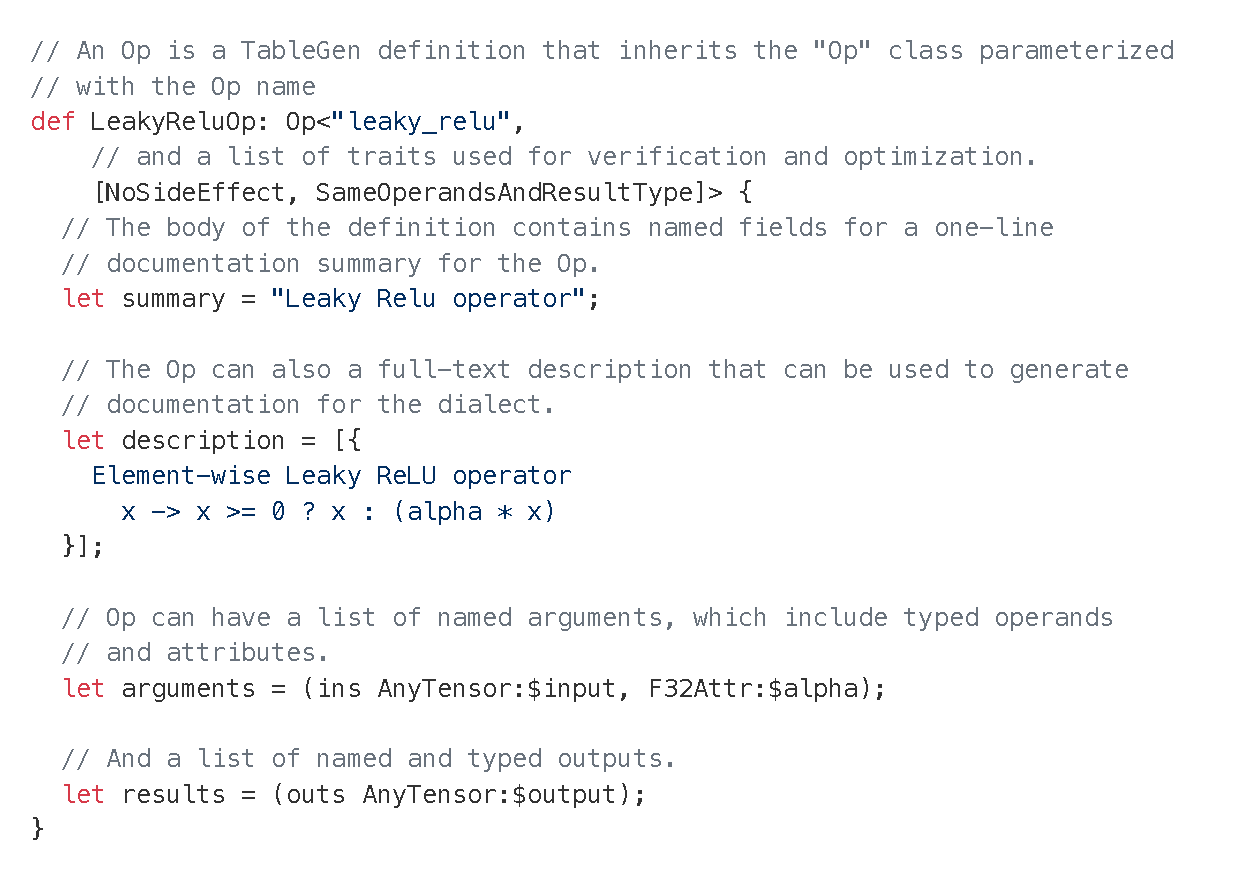
\includegraphics[width=.8\textwidth]{img/leaky_relu.pdf}
  \caption{Operation Definition Syntax (ODS) provides a concise way of defining
        new Ops in \MLIR. Here, one defines the \lstinline|LeakyRelu| Op taking
        a tensor and a floating-point value, and returning a tensor of the same
        type as the input one.}
  \label{fig:ods}
\end{figure}

Ops are modeled in ODS using the  TableGen \lstinline|Op| class.
Figure~\ref{fig:ods} shows an example of Op ODS definition.
Each defined Op has a \emph{name} which is
a unique identifier, a list of \emph{traits} that describe Op properties, a list of
\emph{arguments} that specify Op's operands and attributes, and a list of Op's \emph{results}.
Arguments and results have names and type constraints (e.g., fixed-shape tensor of
\lstinline|float| or \lstinline|int32|). Op definition may also specify
human readable Op description for the documentation.
And a (limited) custom textual form for which custom printer/parser will be generated.
When Op definition
requires finer-grain control than ODS provides, additional \Cpp code can be
injected via \emph{builder}, \emph{printer},
\emph{parser}, \emph{verifier} clauses.
Op traits can be generic, e.g., ``has no side-effects'', and
dialect- or ODS-specific, e.g., ``has custom exporter''.
Traits in ODS may be
backed by \Cpp classes defining the behavior of the trait. There is no fixed
set of traits, but some traits are known by ODS (e.g., ``shape result and
operand type'' represents a constraint that fully captures the output type given
input types) or optimizers (e.g., ``has no side-effects'',
see~\secref{interfaces}).

Type constraints check properties of the type of arguments/results and are
user/dialect extensible. \MLIR infrastructure also provides numerous pre-defined
type constraints, such as ``any type'', ``tensor with element satisfying the
given constraint'', ``vector of given rank'', etc. ODS also has limited support
for automatically deducing the return type of results of operands using the
constraints induced by the traits, see~\secref{drr} for more information.

\subsection{Declarative rewrites}\label{sec:drr}

Many \MLIR transformations involve Op manipulations, and while some
transformations require complex modifications of the IR, many others can be
expressed as simple rewrites on the DAG defined by SSA use-def relations.  \MLIR provides a graph
rewriting framework complemented with the Declarative Rewrite Rule (DRR) system
that makes it simple to express patterns.

Similarly to ODS, DRR is a DSL embedded into the TableGen language. DRR
expresses source and target DAG patterns along with constraints (including
dynamic constraints~\cite{Thier:2018:FFI:3178372.3179501}) and
benefits for pattern prioritization. Patterns can capture and reuse arguments
of an Op.  Conceptually, DRR expresses equivalence of DAGs under specific
constraints. \figref{rewrite} gives an example of a DRR pattern that converts
an Op defined in \figref{ods} into common lower-level implementation consisting
of a \lstinline|compare| and a \lstinline|select|.

\begin{figure}[t]
  \centering
  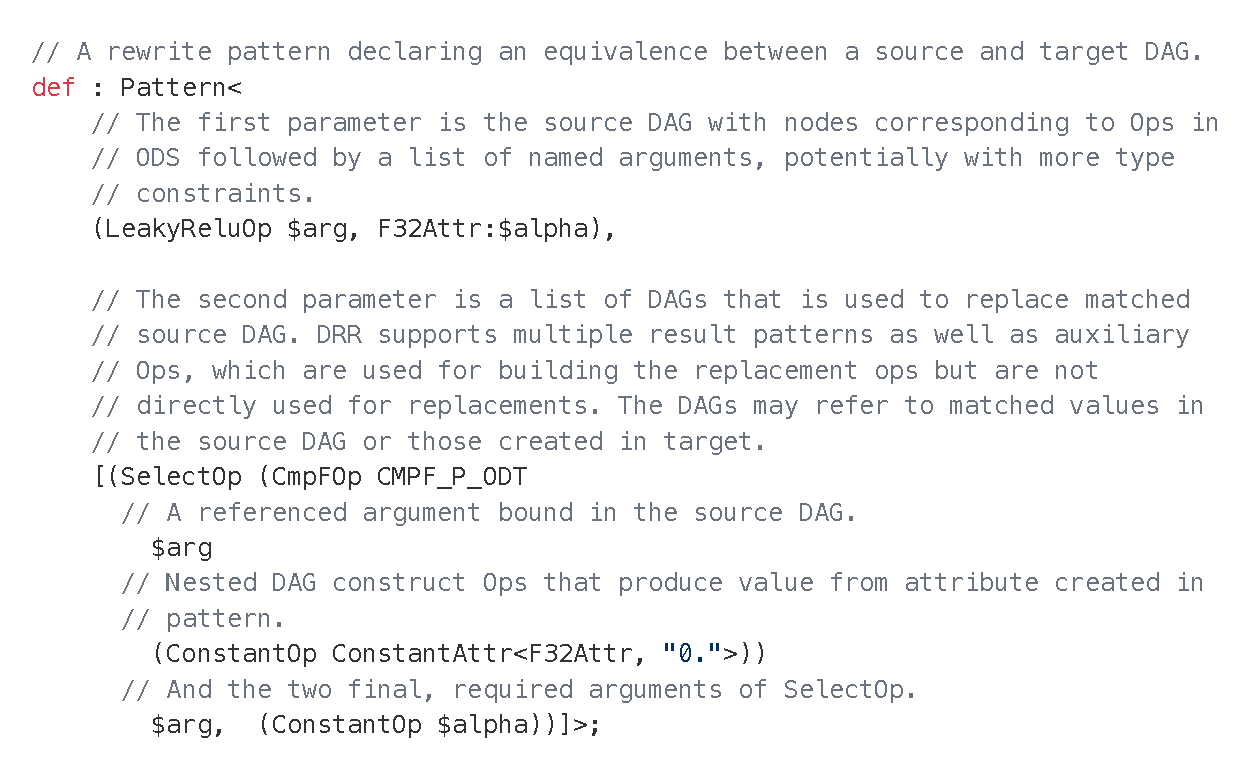
\includegraphics[width=.8\textwidth]{img/pattern.pdf}
  \caption{Declarative graph rewrite rule transforming a LeakyRelu into a
    Compare-Float, followed by a Select.}
  \label{fig:rewrite}
\end{figure}

DRR is converted into \Cpp code, which can be intermixed with more complex
patterns defined directly in \Cpp using the generic graph rewriting framework. This
ability allows \MLIR to keep the common case simple without restricting
generality of the framework.

\subsection{Pass manager}

The \MLIR pass manager organizes and handles the efficient execution of a series
of \emph{IR passes} operating on various granularities.  Whereas pass management
in existing systems is typically defined over a fixed granularity (e.g., module,
function or loop pass managers), in \MLIR modules and functions are not special---they are merely Ops with regions and there can be
multiple variants of them. Therefore, the \MLIR pass manager is also not
specialized on a fixed set of ops, but instead works on arbitrary Ops at
arbitrary levels of nesting.

\paragraph{Parallel compilation}\label{sec:parallel_comp}

An important requirement of \MLIR is the need to utilize multi-core
machines for faster compilation.  The pass manager supports
concurrent traversal and modification of the intermediate representation,
which is made possible by invariants provided by ``isolated-from-above''
property of operations, because the SSA use-def chains cannot cross the
region boundaries of these ops.  Operations with this behavior (e.g. the
``std.func'' operation) thus define a tree of regions that may be
processed in parallel.

This requirement is the reason why (in contrast to, for example, LLVM),
\MLIR does not feature whole-module use-def chains.  Global objects
are referenced through symbol table entries, and constants are implemented
as operations with associated attributes.

\subsection{Round-trippable textual IR form}\label{sec:roundtrippable}

The IR and Ops in \MLIR have a textual representation that fully reflects
the in-memory representation, which is critical for debugging, understanding
the IR during transformations, and for writing test cases.  The
raw IR form shown in \figref{generic} is verbose and difficult to understand.
Therefore \MLIR allows for defining custom printing and parsing formats for Ops,
which allows the example to be printed and parsed as shown in \figref{affine},
which is much easier to work with.

Both forms are fully round-trippable and each compiler pass may be tested
separately, using the textual form as both input and output. Since there is
no hidden state, the
result of running an individual pass is identical to running the same pass in
the full pass pipeline. This approach is user-friendly, as the IR form can be
created by hand, and IR transformations are easy to trace.

\subsection{Documentation}
Dialects, Ops and Interfaces have a documentation generated from their ODS
descriptions. Beyond one line \emph{summary} and more readable
\emph{description}, the generated documentation includes argument and result
type constraints. As the same source is used for both the verification code and
documentation, the documentation has higher changes of remaining in sync with
runtime behavior.

\subsection{Verifiers}

\emph{Verifiers} are used to enforce structural correctness
of the IR and invariants of Ops, allowing passes to assume a verified IR with
invariants checked, and also serves as a debugging tool. Verification
starts with checking structural properties of \MLIR overall: types must match
exactly, values are defined only once and obey dominance and visibility, symbol
names are unique in the symbol table, all blocks end with
terminator Ops, etc. After that, individual Op and attribute verifiers are applied.
Each Op may define a set of structural and semantic rules that check its
validity. For example, a binary Op checks that it has two operands, many Ops
only accept values of specific types, and many require specific
attributes or regions attached. Similarly, dialect attributes can be only
allowed on specific Ops or impose further restrictions on the Ops to which they
are attached. For example, a dialect attribute can require an Op to only use
types defined in the dialect even though the Op itself is more generic.
Verification failures are considered invariant violations and abort compilation.
